\subsection{Numerical Examples and Their Implications}\label{sec:network:performance_model:numerical_examples}

%TODO: Introduction

\subsubsection*{Model Validations}\label{sec:network:performance_model:validations}

In order to assess the applicability of our performance model, we first have to check whether real-world application traces can be modeled as renewal process, which was our main assumption for the model.
We use the Lewis-Robinson-Test \cite{Ascher1984}, which is a hypothesis test with null hypothesis \(H_0\) that the tested process is a renewal process.
To this end, we use exemplary the measurement, obtained with the measurement testbed introduced in \refsec{sec:network:network_traces:performance_evaluation:measurement}, for two different types of applications: \emph{Twitter} and \emph{K9-Mail}.
According to this test, the null hypothesis cannot be rejected for both of our packet traces at a significance level of \SI{95}{\percent}.
Although this assumption may not be true for all applications, our results show that at least the considered applications can be modeled as a renewal process.

Next, we compare our analytical performance results with \gls{RRC} protocol simulations using measured application and \gls{TCP} traces which are described in more detail in \refsec{sec:network:network_traces:numerical_results:traffic_characterization}.
In order to produce analytical results that correspond to the real applications, we extract the empirical distributions of the inter-packet time \(\PacketIAT\) from the traces for both applications and use these distributions as input for \refeq{eq:network:performance_model:system_description:state_distribution:observation_density}. 

In \reffig{fig:network:performance_model:numerical_examples:validations:analytic_vs_simulation} we compare the accuracy of the results  obtained by the presented method to the values obtained from simulations for the two measured applications and both considered metrics.
We observe that the accuracy for both power drain \(\gls{PD}\) and \(\gls{SI}\) is very high.
In \reffig{fig:network:performance_model:numerical_examples:validations:analytic_vs_simulation:signalling_intensity} the results for both the Mail and Twitter application obtained by the model completely align with the signalling intensity obtained by the simulation.
The comparison of analytical results for the power drain to the simulation in \reffig{fig:network:performance_model:numerical_examples:validations:analytic_vs_simulation:power_drain} leads to the same conclusions as for the signaling intensity.

\begin{figure}
	\begin{subfigure}[b]{\textwidth}
	\centering
	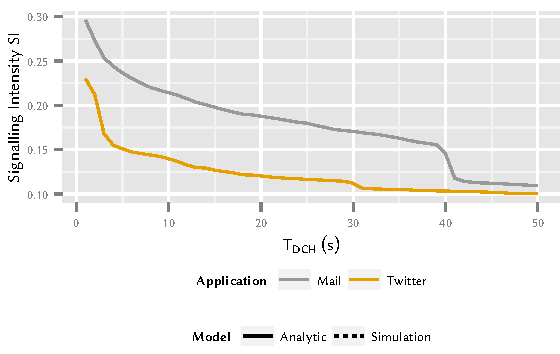
\includegraphics{network/performance_model/numerical_examples/figures/3state_tdch_si_analytic_simulative}
	\caption{Signalling Intensity}\label{fig:network:performance_model:numerical_examples:validations:analytic_vs_simulation:signalling_intensity}
	\end{subfigure}

	\begin{subfigure}[b]{\textwidth}
	\centering
	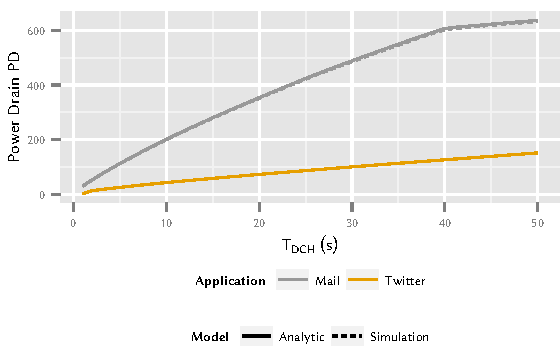
\includegraphics{network/performance_model/numerical_examples/figures/3state_tdch_pd_analytic_simulative}
	\caption{Power Drain}\label{fig:network:performance_model:numerical_examples:validations:analytic_vs_simulation:power_drain}
	\end{subfigure}

	\caption{Comparison of the Performance Model with \glsshort{3G} Simulation for the Three State Scenario}\label{fig:network:performance_model:numerical_examples:validations:analytic_vs_simulation}
\end{figure}

\subsubsection*{Impact of Traffic Patterns on Signaling Intensity}\label{sec:network:performance_model:signaling_intensity}
First, we focus on the signaling intensity \(gls{SI}\) of traffic patterns and check the impact of the average inter-packet time \(E[\PacketIAT]\) and the timer configuration. The signaling intensity \(\gls{SI}\), i.e., the average number of state transitions required for the transmission of a single packet, is an abstract measure for the signaling load produced by a specific traffic pattern.

\paragraph*{Impact of the Average Inter-Packet Time \(E[\PacketIAT]\)}
Some applications, for example those downloading or streaming of videos, send and receive large amounts of data within short time frames.
In contrast, other applications such as social network clients send and receive small amounts of data every few minutes over the time span of some hours or days.

In this section we study the impact of average inter-packet times \(E[\PacketIAT]\) and the burstiness of the traffic pattern, i.e., the coefficient of variation 
\[c_{\PacketIAT} = \frac{\sqrt{\mathrm{Var}[\PacketIAT]}}{\mathrm{E}[\PacketIAT]}\]
 on the signaling load.
For that purpose, we use the simple two state scenario, set the timer \(\gls{TDCH}=\SI{10}{\second}\), consider only the first and the second moment of the inter-packet time \(\PacketIAT\), and assume that \(\PacketIAT\) follows a lognormal distribution, where both moments can be varied independently.

\subsubsection*{Impact of Traffic Patterns on Power Drain of the \headershortacr{UE}}\label{sec:network:performance_model:power_drain}
\subsubsection*{Trade-off: Energy Consumption vs. Signalling Load}\label{sec:network:performance_model:trade_off}
